\documentclass[a4paper]{article}
\usepackage[utf8]{inputenc}
\usepackage{graphicx}
\graphicspath{{./Bilder/}}

\title{Spillmanual for SPOOKS - Skummelt Pek og Ondskapsfullt Klikk Spill}
\author{INF112-TEAM1\_2}

\begin{document}
\maketitle

\tableofcontents
\pagebreak

\subsection{Vår idé} Vi ønsker å lage et skrekkbasert pek-og-klikk spill. Målet med spillet er at spilleren skal komme seg ut av et skummelt hus. Dette oppnås ved at spilleren løser forskjellige gåter og oppgaver slik at flere dører til nye rom åpnes i huset. Når spilleren har løst alle gåtene og oppgavene vil spilleren kunne forlate huset og spillet er over. Vi ønsker at gåtene og oppgavene skal variere mellom alt fra å finne nøkler, kombinere ulike gjenstander, til å løse små hjernetrims spill; alt under tidspress. Hvert femte minutt mister spilleren alle gjenstandene sine og starter fra siste checkpoint. Dette vil si at spilleren kanskje ikke alltid har tid til å plukke opp alle gjenstandene som går an å bruke, men lærer til neste hvilke gjenstander det er verdt å ta med seg til den oppgaven som skal utføres. Vi ønsker også at oppgavene skal være utfordrende og stige i vanskelighetsgrad etter hvert som spilleren kommer videre i spillet. Vi ønsker også at spilleren skal kunne lagre spillet og dermed ha muligheten til å kunne fortsette spillet på et annet tidspunkt.

\subsection{Målgruppe}
Spillet er ment for personer som liker skrekkspill. Forløpig er det vanskelig å sette en aldersgrense i og med at vi ikke vet hvor skummelt spillet blir, men vi håper at vi kan sette en aldersgrense og sikte til en målgruppe på 12+ år.

\subsection{Spilletid}Spilletiden avhenger av Spillerens egenskaper til å løse gåter/oppgaver. Hvis spilleren har løst mange lignende gåter og/eller oppgaver vil spilletiden minskes og vice versa. 
Spillet er lagt opp til å resette seg hvert 5-10 minutt. Det vil si at man må rekke neste checkpoint innen 
5 minutter ellers starter man fra forrige checkpoint i spillet. Spilletiden vil også avhenge av hvor omfattende spillet blir. Spillet skal kunne lagres, slik at Spilleren kan starte spillet fra sist lagrede punkt.

\subsection{Gamemode}
Spillet er et en-spiller spill, hvor Spilleren spiller som førsteperson. Det vil si at spilleren vil se omgivelsene gjennom karakterens øyne.

\subsection{Brukerfortellinger}
\begin{itemize}
\item Som spiller vil jeg kunne klikke på ting og forvente at det skjer noe om jeg gjør noe riktig.
\item Som spiller ønsker jeg å få hint hvis det går lang tid uten at det skjer noe eller at jeg ikke klarer å løse en oppgave.
\item Som spiller vil jeg at spillet gir meg en beskjed hvis jeg gjør noe feil.
\item Som spiller vil jeg å kunne avslutte og lagre spillet når som helst og fortsette videre på et annet tidspunkt.
\item Som spiller vil jeg at spillet skal være selvforklarende og enkelt å forstå.
\end{itemize}

\section{Bruksmønster}

\begin{raggedright}
{\bf Overview:} Spillet starter, du befinner deg i et hus. Du vet ikke hvor du er, og må komme deg ut av huset.\\
{\bf Actors:} Spiller, Maskin\\
{\bf Pre-conditions:} Ingen\\
\end{raggedright}

\subsection{Hovedcase}
\begin{enumerate}
\item Meny (Start – slutt)
\item Spiller velger å starte ett nytt spill
\item Systemet oppretter et nytt spill
\item Systemet starter en klokke som teller ned fra 5minutter
\item Spiller trykker på et element i spillet
\item Systemet gjør noe med elementet
\item Spiller belønnes med å få en ting
\item Systemet legger tingen i Spillerens inventory\\

\textit{Steg 4-7 går i loop til Spiller har nøkkel til å gå videre neste rom}
\item Spiller velger ''nøkkel'' fra inventory
\item Systemet markerer ''nøkkel'' i inventoryen
\item Spiller trykker på dør
\item Systemet åpner døren
\item Spiller klikker på døren
\item Systemet flytter spilleren til neste rom (nivå)\\

\textit{Steg 4-13 går i loop til Spiller har funnet ''master key''}
\item Spiller plukker opp ''master key''
\item Systemet legger ''master key'' i inventory
\item Spiller velger ''master key'' fra inventory
\item Systemet markerer ''master key'' i inventory
\item Spiller klikker på utgangsdøren
\item Systemet åpner døren
\item Systemet forteller Spilleren at Spiller vant
\item Systemet returnerer til hovedmeny
\end{enumerate}

\subsection{Alternative hendinger}
\begin{itemize}
\item[A1] @2 Spiller velger å avslutte spillet
\item[A2] Systemet avslutter spillet
\item[B1] @4 Spiller prøver å åpne en dør som er lukket
\item[B2] Systemet gir Spiller beskjed om at døren er låst
\item[C1] @4, 6, 8, 10, 12, 14, 16, 18 stoppeklokken går ut
\item[C2] Systemet sletter alt i inventory
\item[C3] Systemet plasserer Spiller i utgangspunktrommet
\item[C4] Systemet starter en klokke som teller ned fra 5 minutter
\end{itemize}

\subsection{Bruksmønsterdiagram}

 \fbox{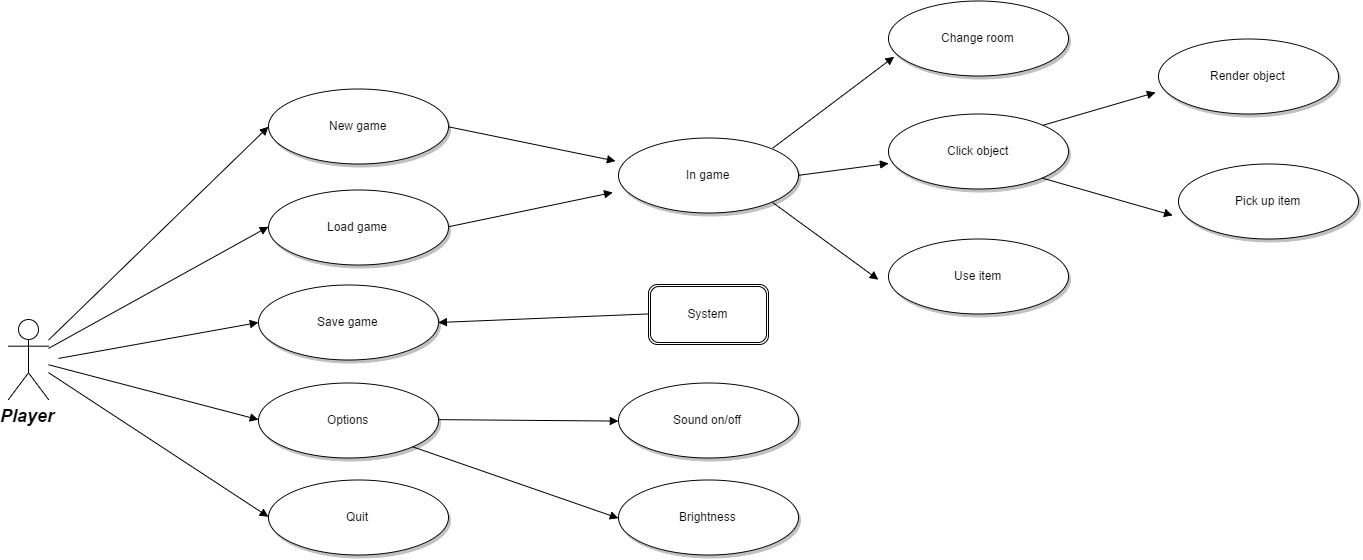
\includegraphics[width=1.02\textwidth]{UML.jpg}}

\subsection{Illustrasjoner}
 
\fbox{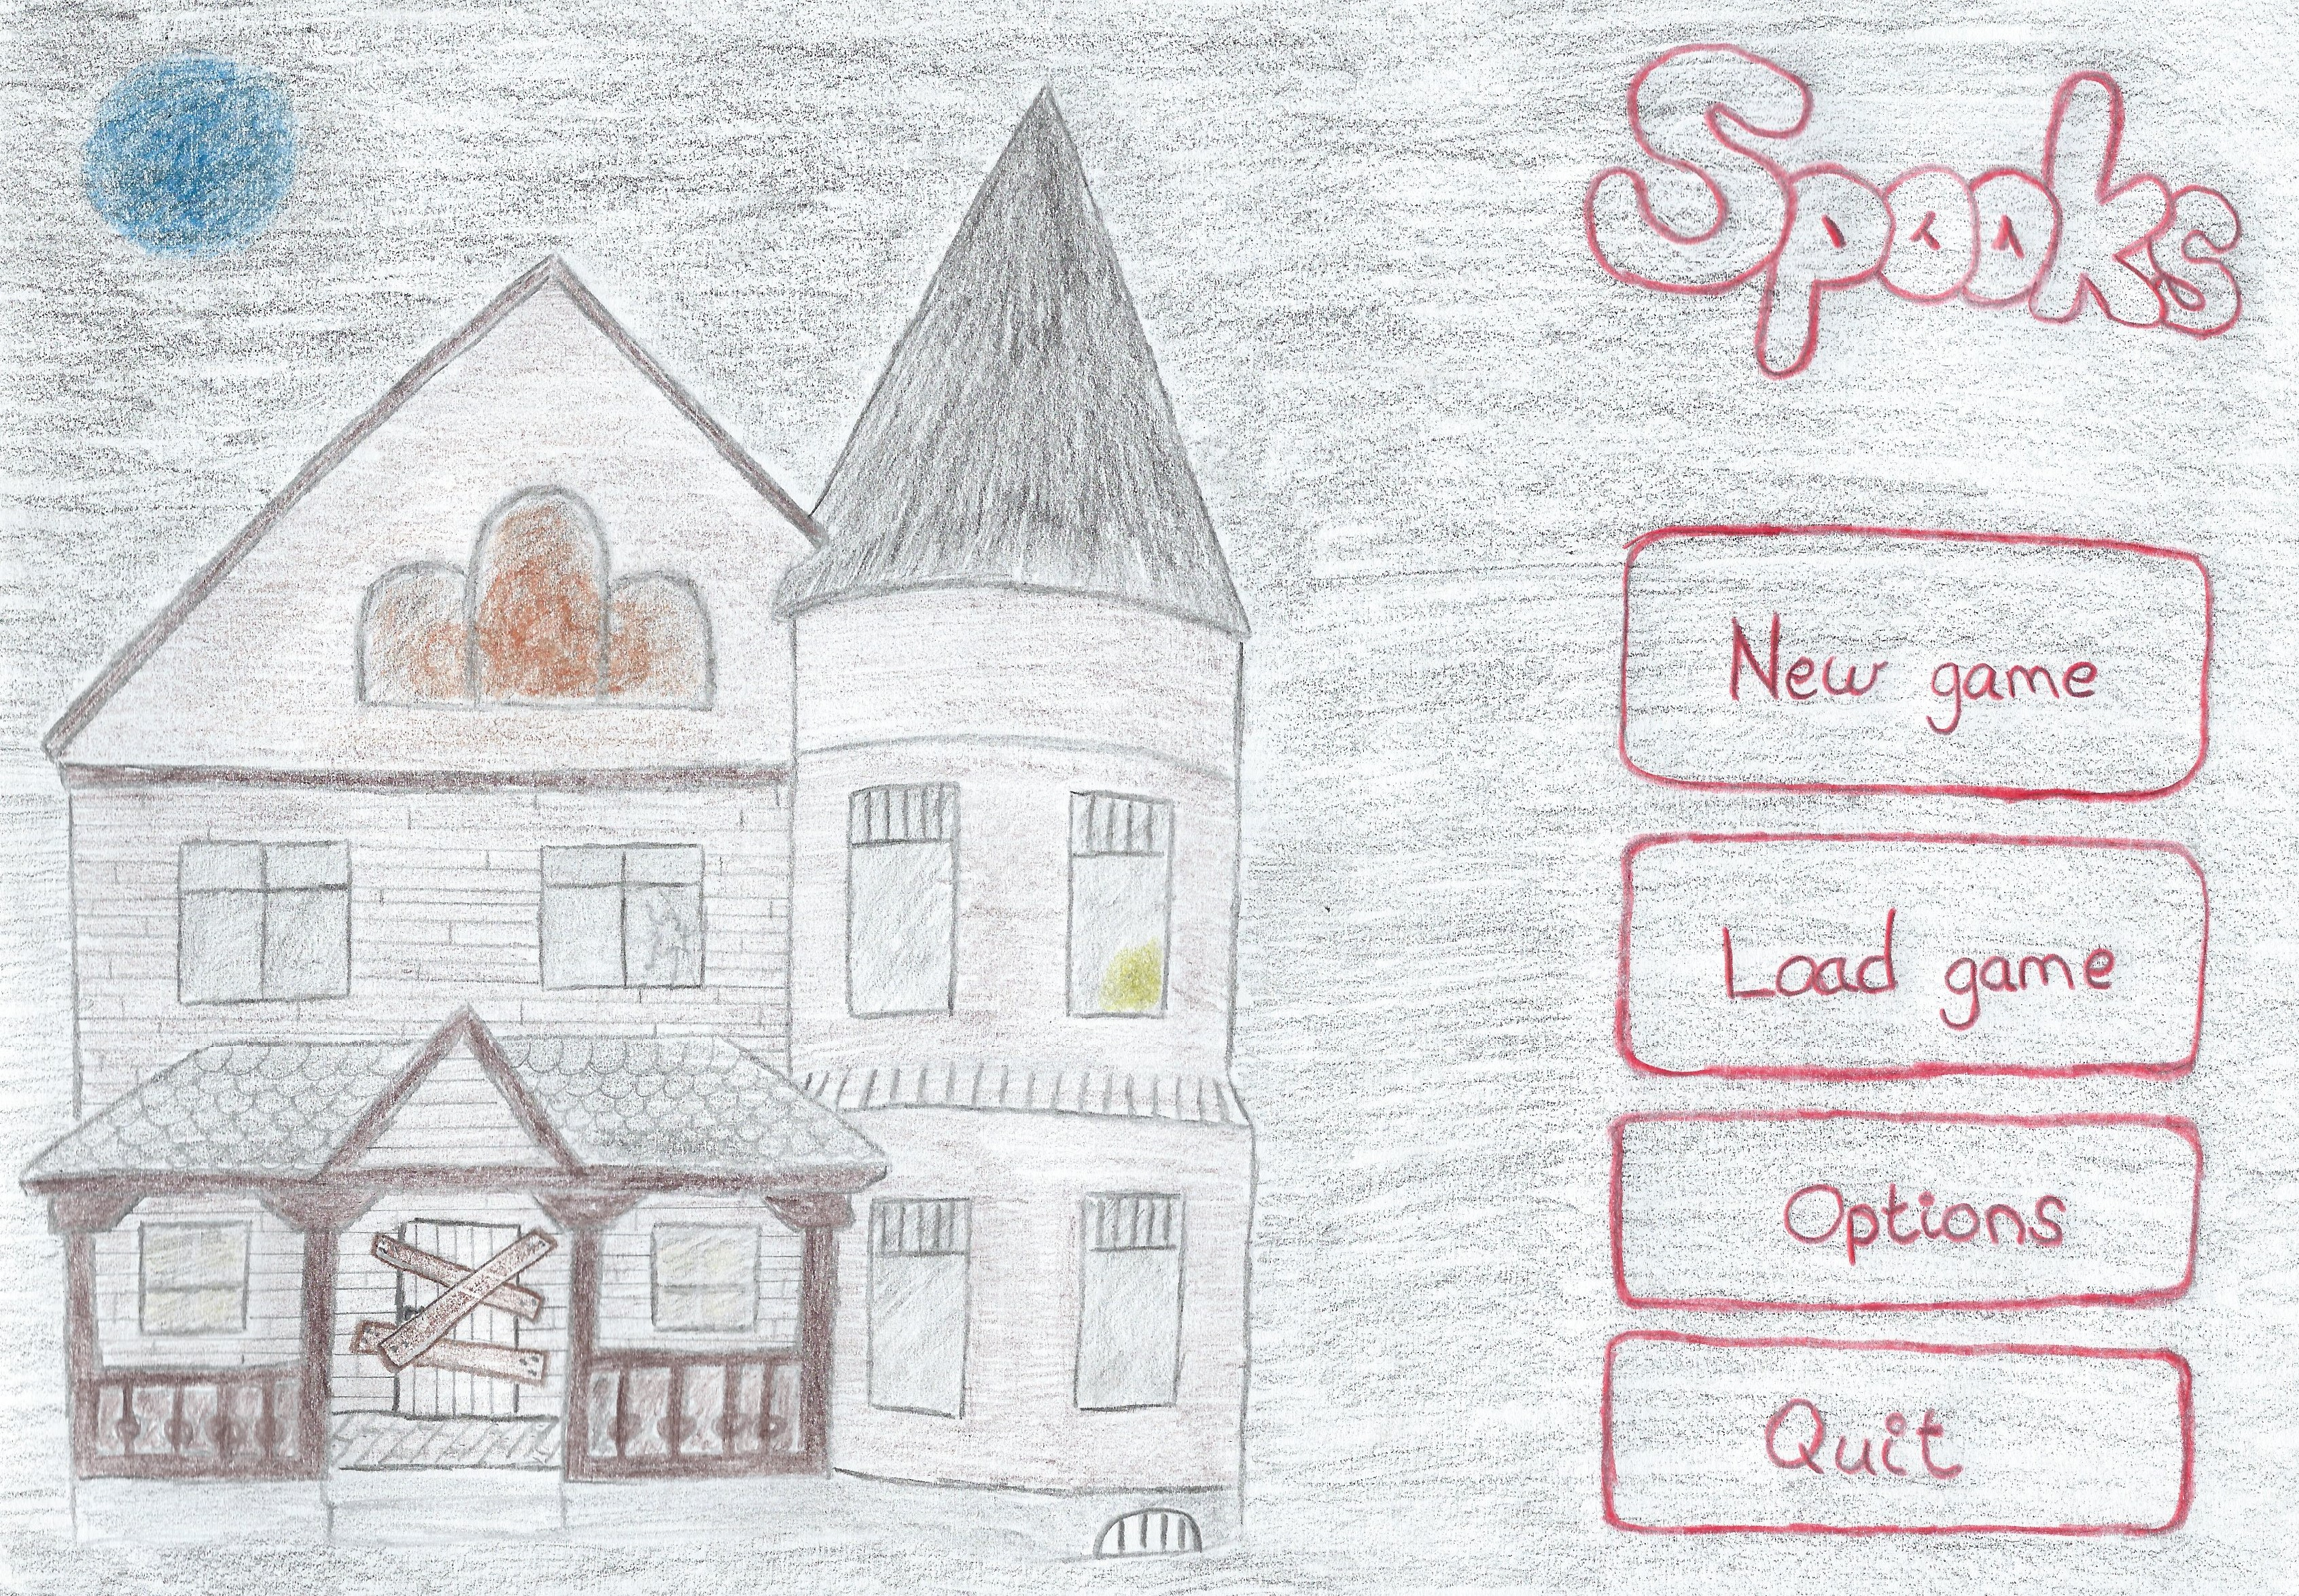
\includegraphics[width=1.02\textwidth]{bilde2.jpg}}
\fbox{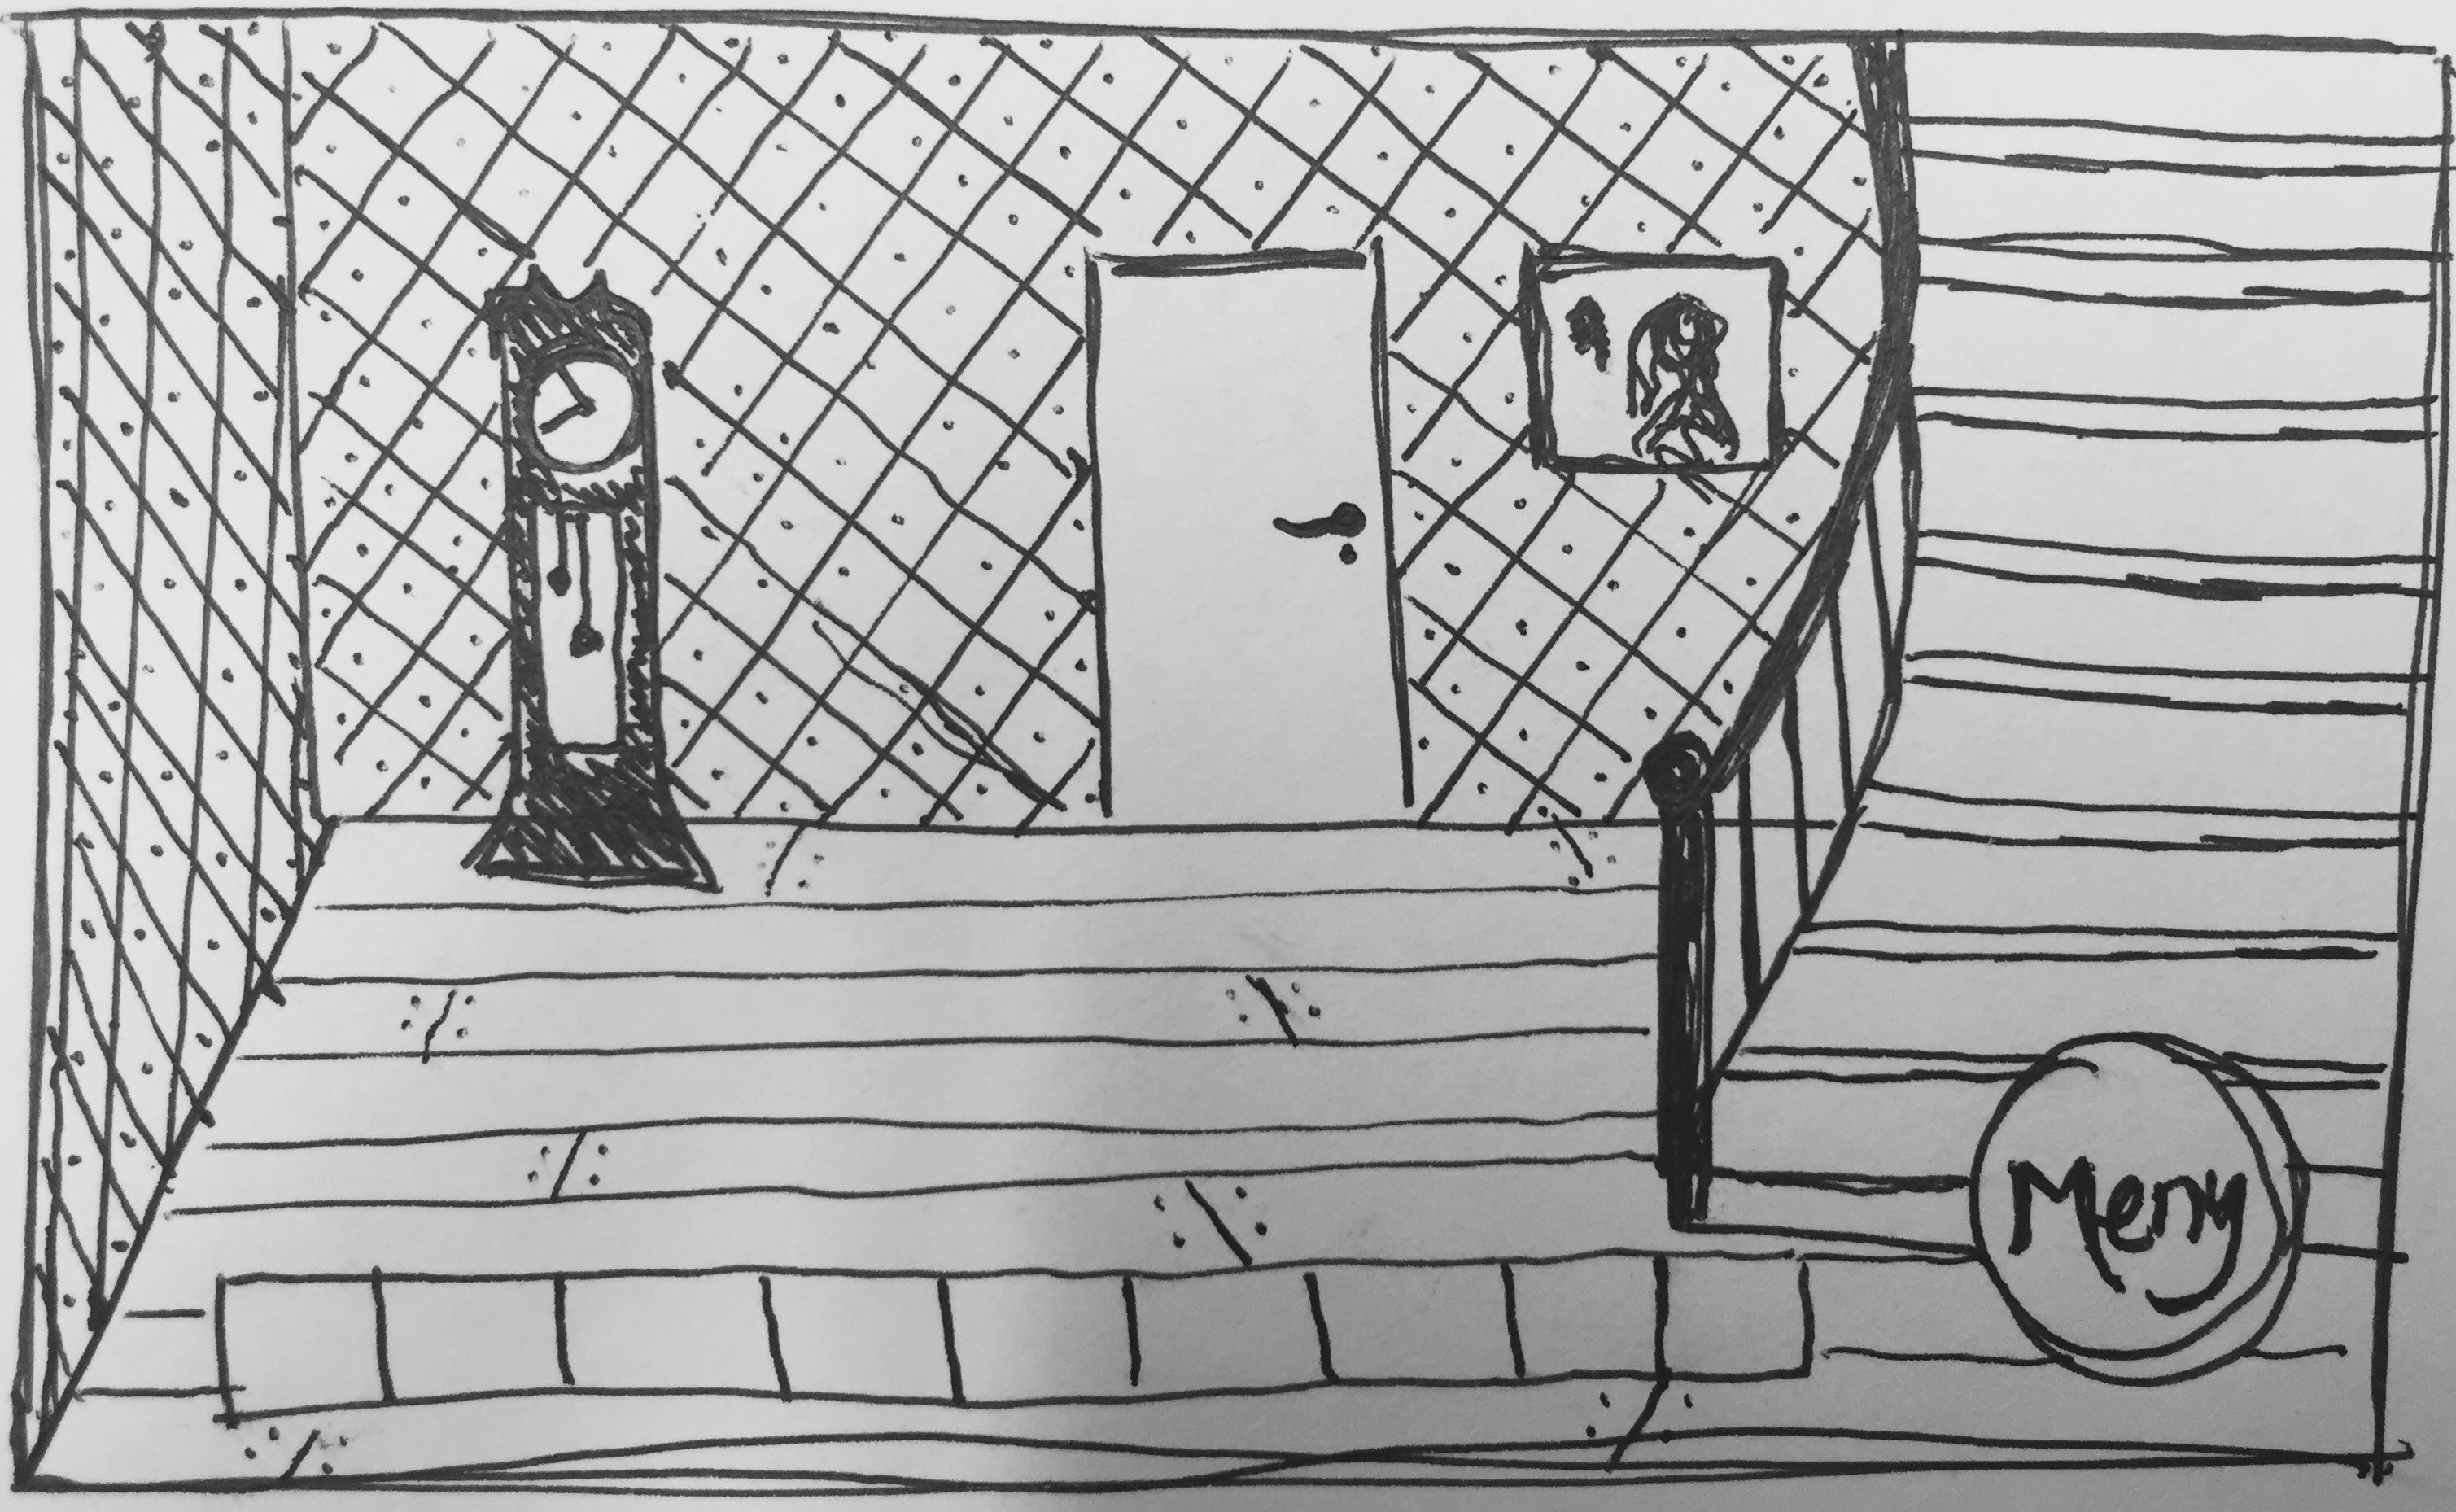
\includegraphics[width=1.02\textwidth]{bilde1.png}}
\fbox{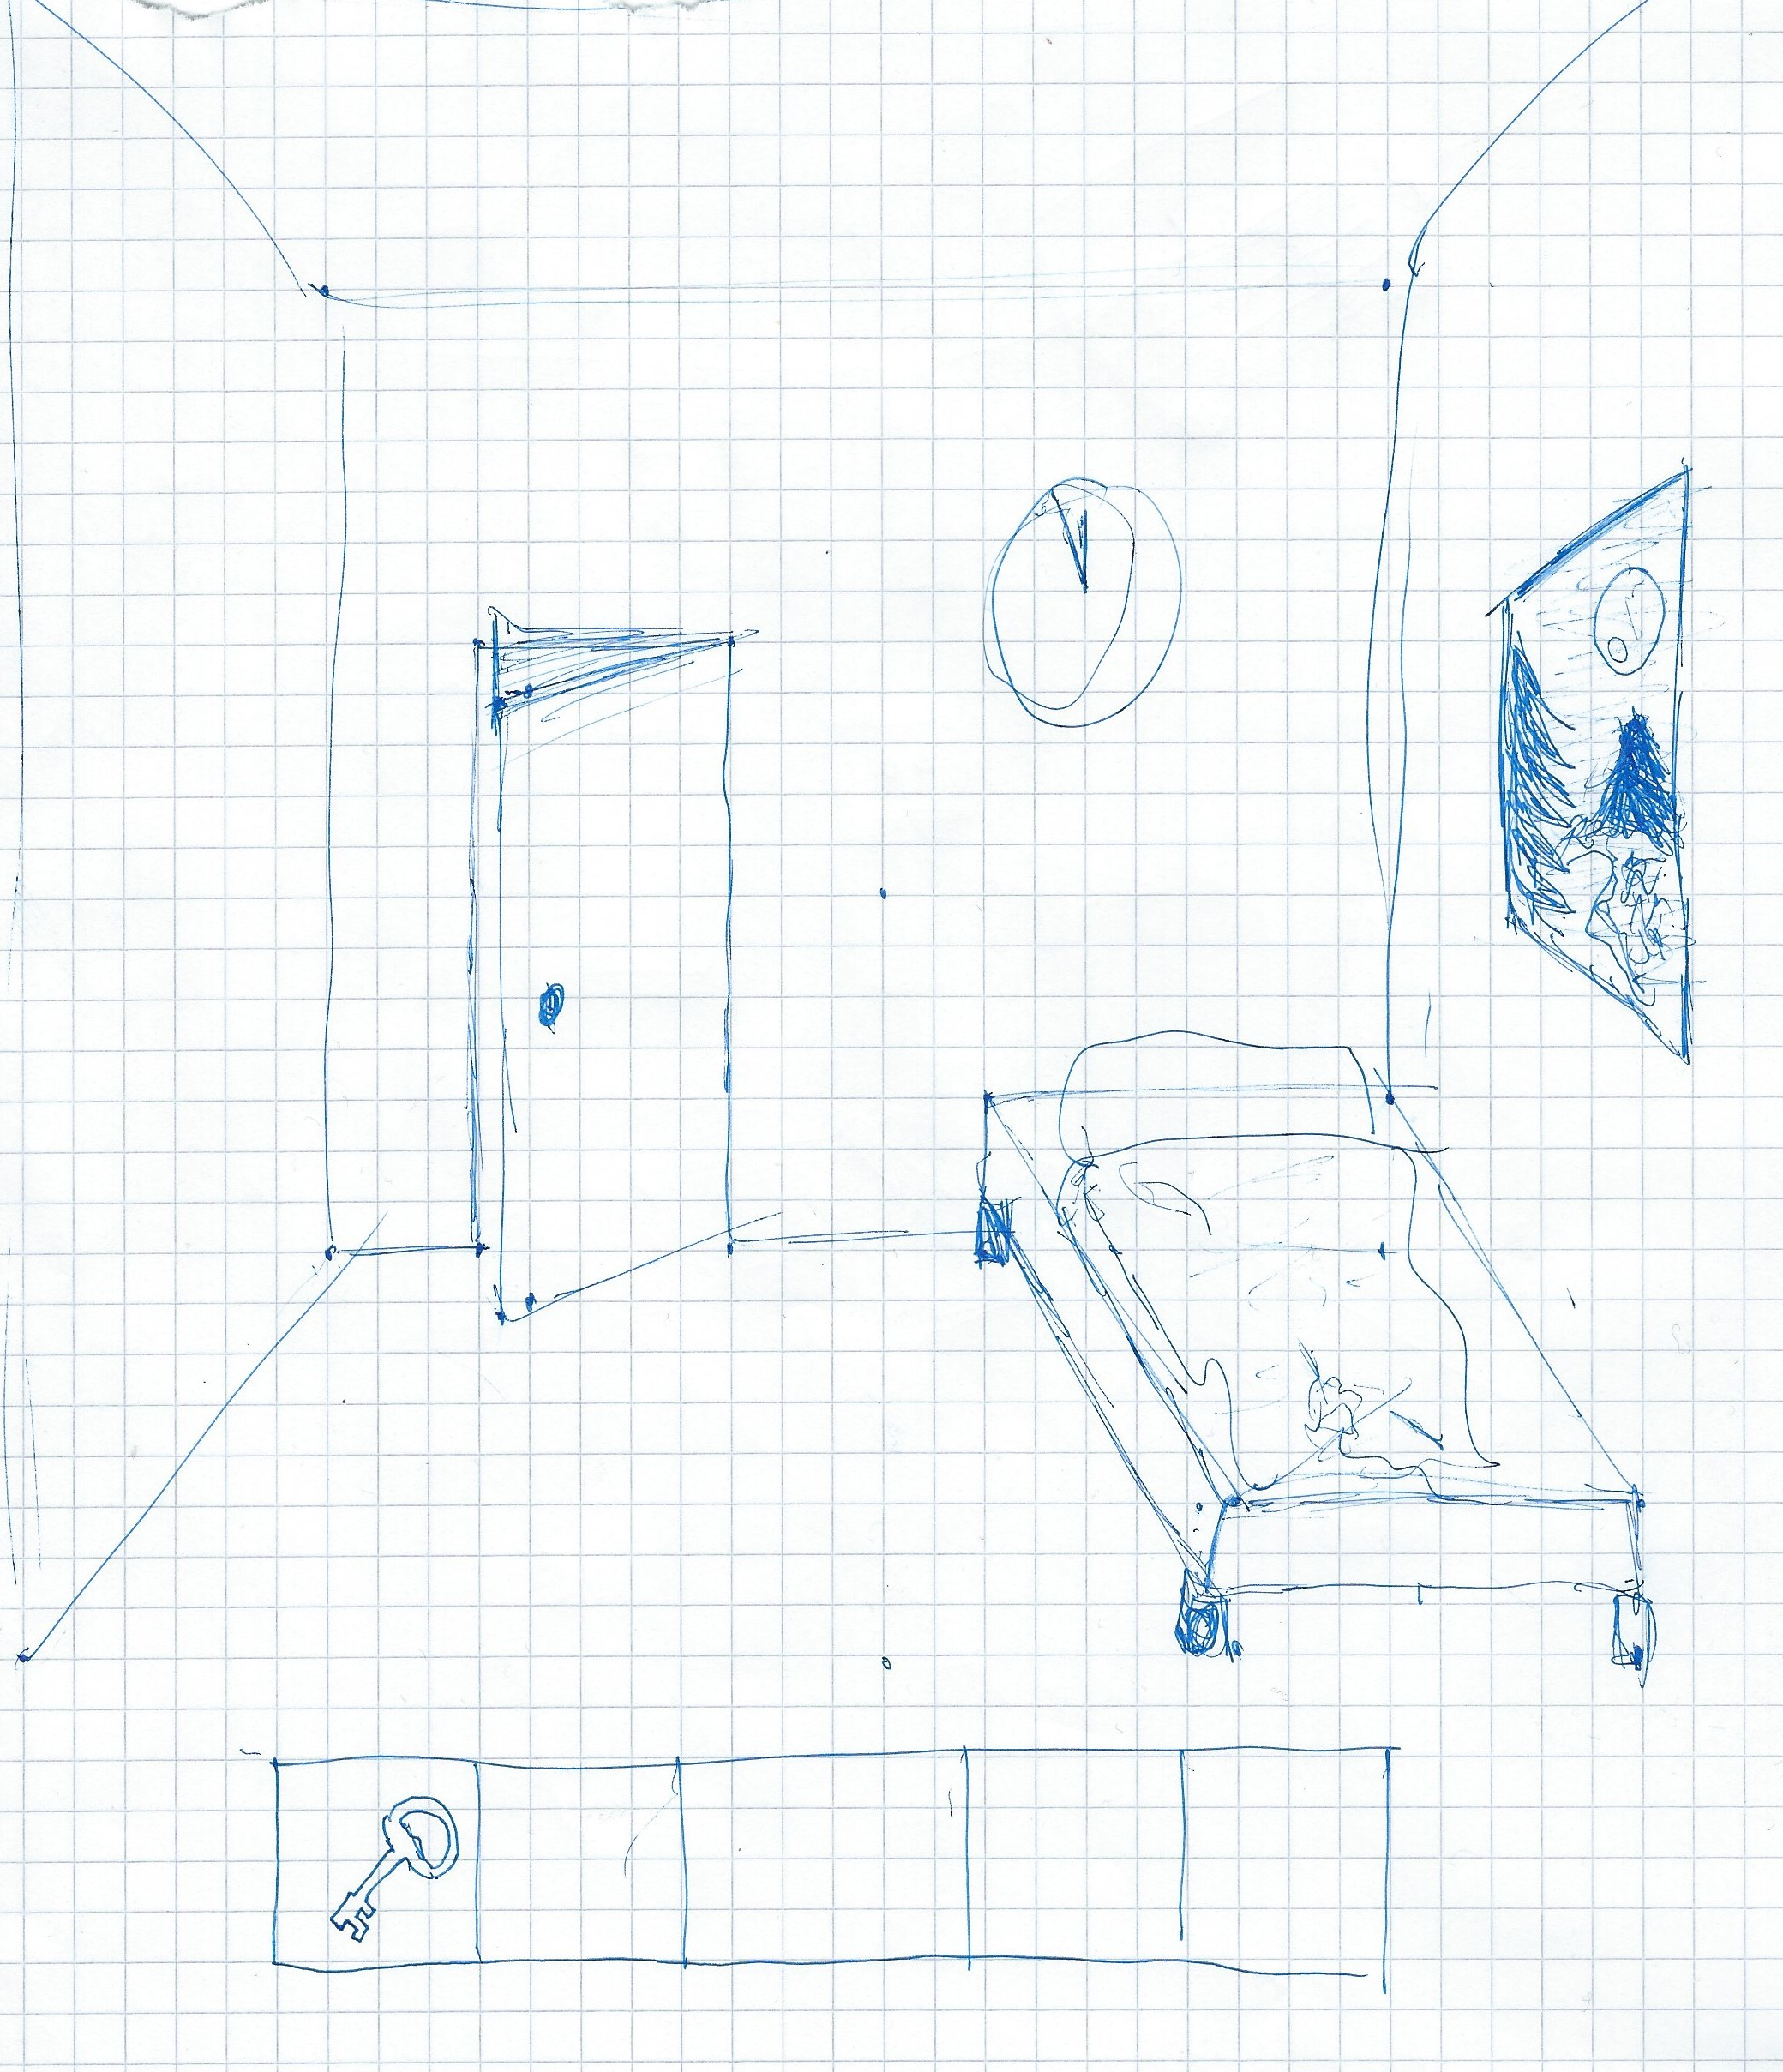
\includegraphics[width=1.02\textwidth]{bilde3.jpg}}

\subsection{Spillregler}

\begin{itemize}
\item Spilleren kan ikke dø i spillet
\item Spillet resettes hvert 5-10 minutt og spilleren vil havne tilbake til siste checkpoint
\item Spilleren kan kun bevege seg til gitte punkter i huset (dette er en stor fordel med pek-og-klikk fordi spilleren ikke nødvendigvis kan bevege seg dit spilleren vil)
\item Spilleren kan plukke opp gitte gjenstander i huset og bruke dem til å løse oppgaver/gåter
\item Spilleren kan lagre spillet når som helst og starte fra lagringspunket ved et annet tidspunkt.
\end{itemize}

\end{document}
